% Copyright (c) Geoffrey Lentner 2015. All Rights Reserved
% LabReport/Source/Methods.tex

\section{Experimental Methods}
I can also include subsections. \blindtext

\subsection{Equipment Setup}
To include a figure within the two column environment use ``Figure''.
To include a figure that spans the two column format, use ``figure*''.
Now I can references my figures as Figure~\ref{fig:Hist1} and
Figure~\ref{fig:fourier}. \LaTeX will decide where to put the 
figures \textit{for me}. 

Some more blank text -- \blindtext

% = = = = = = = = = = = = = = = = = = = = = = = = = = = = = = = = = = = = = = =
% Figure spanning 2 column

\begin{figure*}[!t]
	\captionsetup{width=0.8\textwidth}
	\centering
	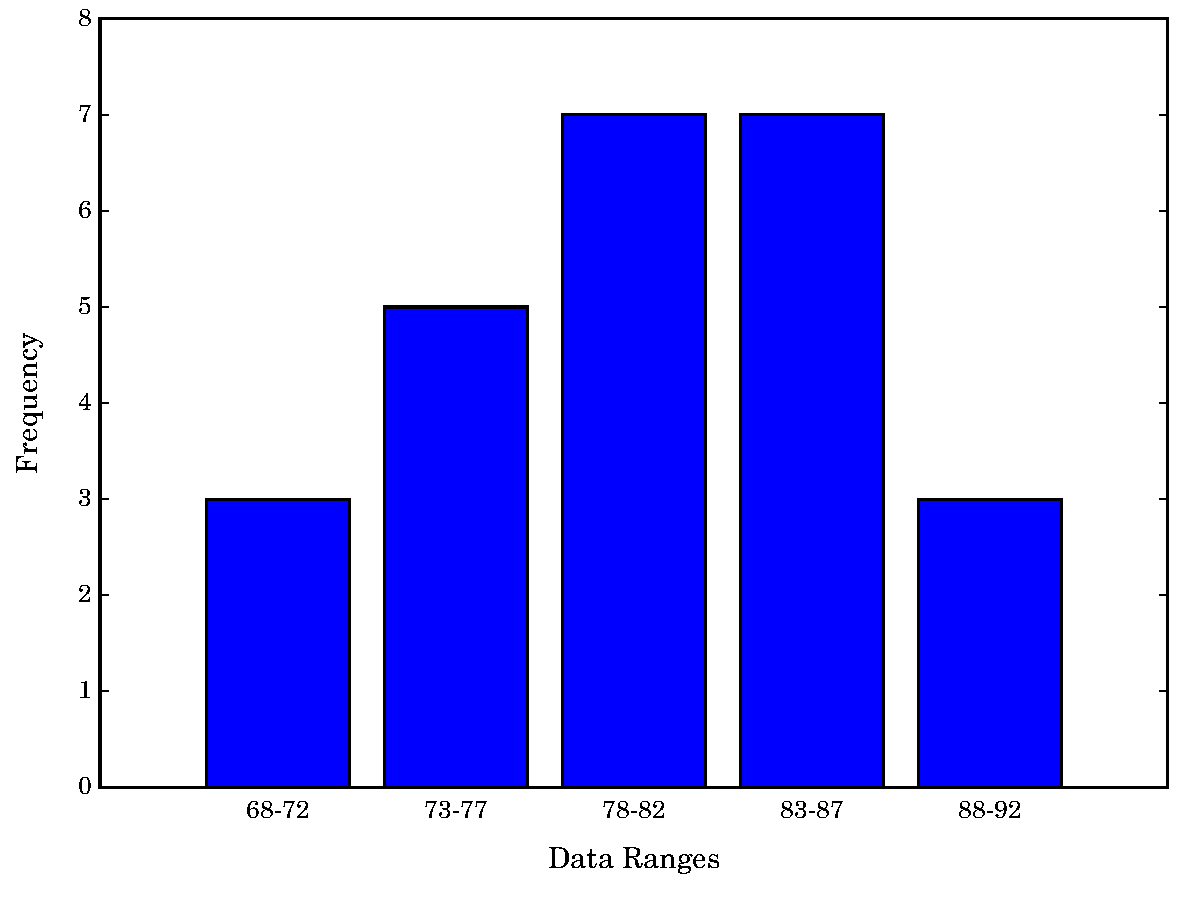
\includegraphics[width=0.8\textwidth]{Figures/Hist1}
	\caption{\blindtext}
	\label{fig:Hist1}
\end{figure*}

% = = = = = = = = = = = = = = = = = = = = = = = = = = = = = = = = = = = = = = =
% Figure with within 2 column

\begin{Figure}
	\captionsetup{width=0.9\textwidth}
	\centering
	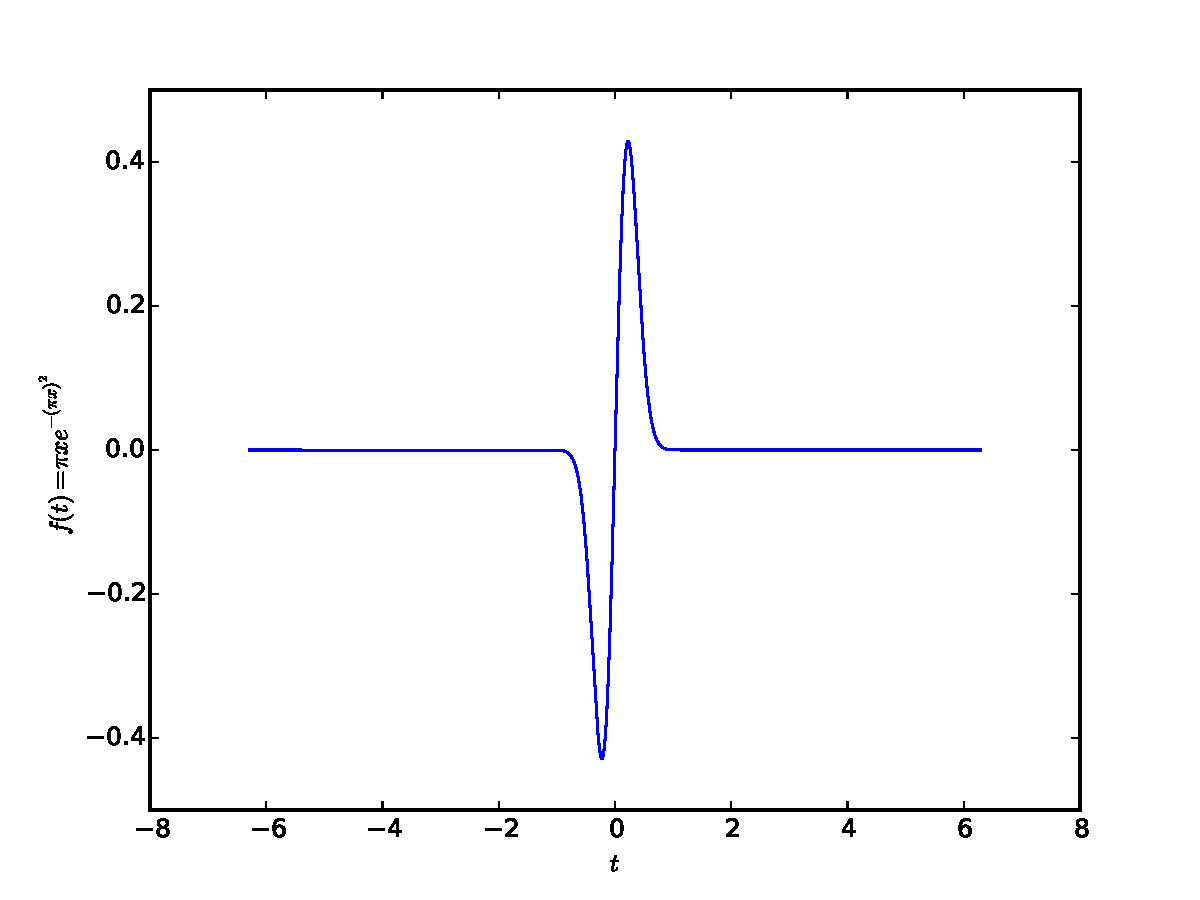
\includegraphics[width=\linewidth]{Figures/hw3.pdf}
	\captionof{figure}{A blind text like this gives you information about the 
	selected font, how the let- ters are written and an impression of the look. 
	This text should contain all letters of the alpha- bet and it should be 
	written in of the original lan- guage. There is no need for special 
	content, but the length of words should match the language.}
	\label{fig:fourier}
\end{Figure}

% = = = = = = = = = = = = = = = = = = = = = = = = = = = = = = = = = = = = = = =
% Figure with two subfigures

\begin{figure*}[!t]
	\captionsetup{width=0.8\textwidth}
	\begin{subfigure}[t]{.49\textwidth}
		\centering
		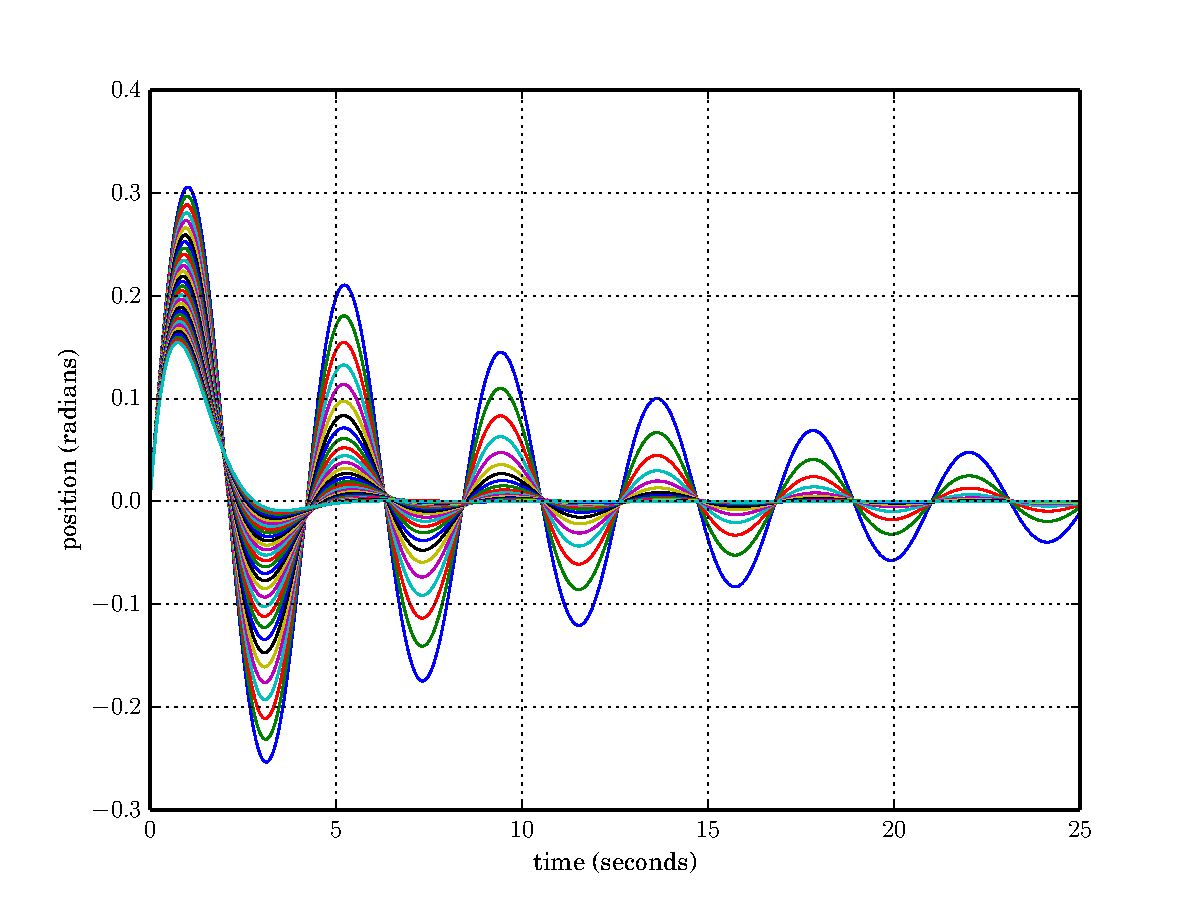
\includegraphics[width=\textwidth]{Figures/plot02.pdf}
		\caption{Variation of Drag Coefficient}
		\label{fig:01A}
	\end{subfigure}
	\begin{subfigure}[t]{0.49\textwidth}
		\centering
		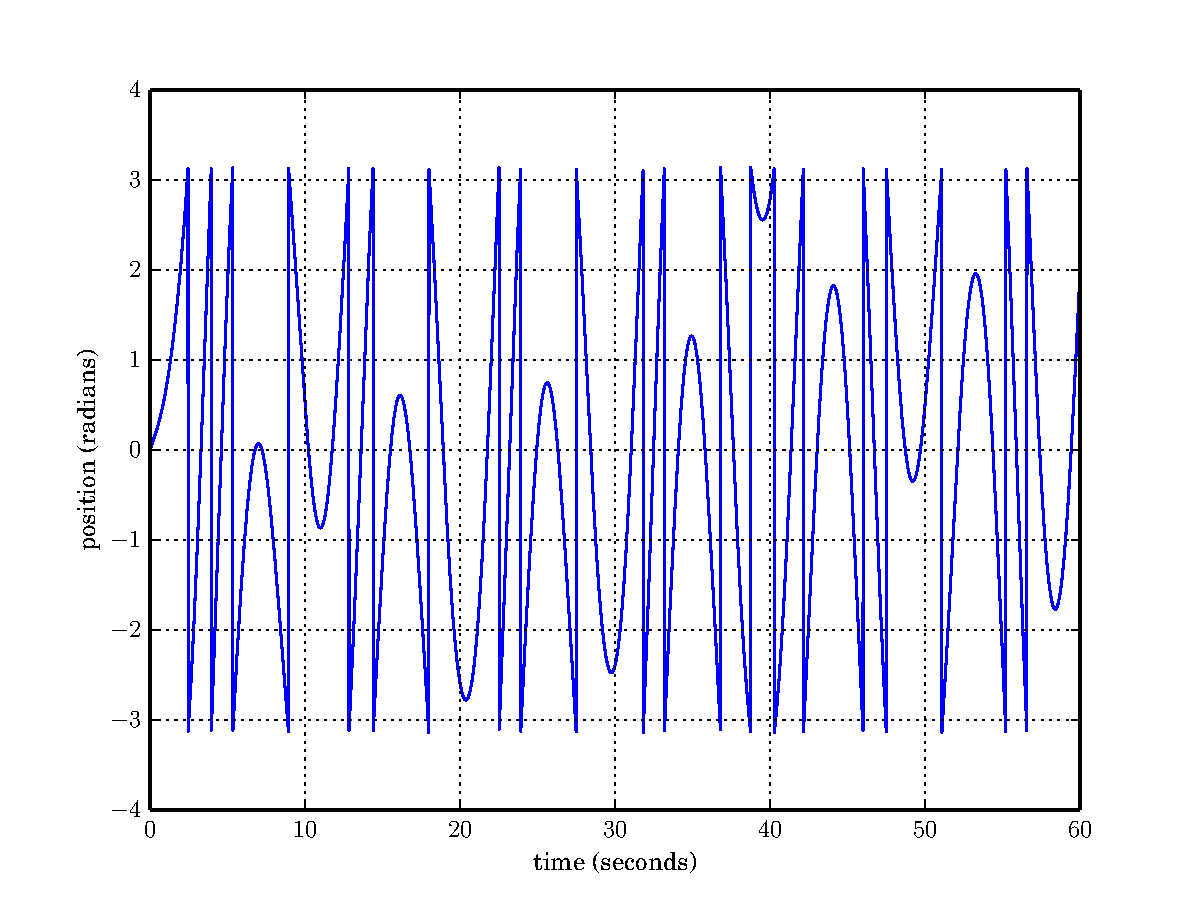
\includegraphics[width=\textwidth]{Figures/plot03.pdf}
		\caption{Variation of Amplitude gives Period Doubling}
		\label{fig:02A}
	\end{subfigure}
	\caption{\blindtext}
	\label{fig:contour}
\end{figure*}

\subsection{Experimental Procedure}
\blindtext[2]